\documentclass[dvipdfmx]{jsarticle}
\usepackage[dvipdfmx]{graphicx}
\usepackage{float}
\usepackage{listings}

\lstset{%
  language={C},
  basicstyle={\small},%
  identifierstyle={\small},%
  commentstyle={\small\itshape},%
  keywordstyle={\small\bfseries},%
  ndkeywordstyle={\small},%
  stringstyle={\small\ttfamily},
  frame={tb},
  breaklines=true,
  columns=[l]{fullflexible},%
  numbers=left,%
  xrightmargin=0zw,%
  xleftmargin=3zw,%
  numberstyle={\scriptsize},%
  stepnumber=1,
  numbersep=1zw,%
  lineskip=-0.5ex%
}

\renewcommand{\lstlistingname}{プログラム}


\begin{document}

\title{アドバンスドCG第1回}
\author{日比野 文}
\maketitle

\section*{課題1}

\begin{lstlisting}[caption=Pathtracer]
		// TODO: implement Lambert (diffuse) reflection with BRDF importance sampling

    // DiuuuseMaterialを取得
    DiffuseMaterial* diffuseMaterial = dynamic_cast<DiffuseMaterial*>(record.m_pMaterial);

    // PIの定義
    const float PI = 3.14159265358979323846f;

    // 拡散反射係数を取得
    const vec3& rho_d = diffuseMaterial->getDiffuseCoeff();

    // ロシアンルーレットの閾値を計算
    const float russianRouletteProbability = (recursionDepth > s_MinRecursionDepth) ? std::max(rho_d.x, std::max(rho_d.y, rho_d.z)) : 1.0f;


    // レイを局所座標系に変換
    vec3 xLocal, yLocal, zLocal;
    calcLocalCoordinateSystem(record.m_Normal, ray.getUnitDir(), xLocal, yLocal, zLocal);

    // 乱数を生成してθとφを決定
    const float u = frand();
    const float v = frand();
    const float theta = 2.0f * PI * u;
    const float phi = acos(sqrt(1.0f - v));

    // 局所座標系での新しいレイの方向を計算
    vec3 newDir = sin(phi) * cos(theta) * xLocal + sin(phi) * sin(theta) * yLocal + cos(phi) * zLocal;

    // 新しいレイで再帰呼び出し(traceRec)
    const vec3 incomingRadiance = traceRec(Ray(record.m_HitPos, newDir), recursionDepth + 1);

    // 反射色を計算
    const vec3 reflectionColor = (rho_d / PI);

    // ロシアンルーレットに従って反射色を修正
    const vec3 weight = reflectionColor / russianRouletteProbability;

    return weight * incomingRadiance;
\end{lstlisting}
\begin{figure}[H]
 \begin{center}
  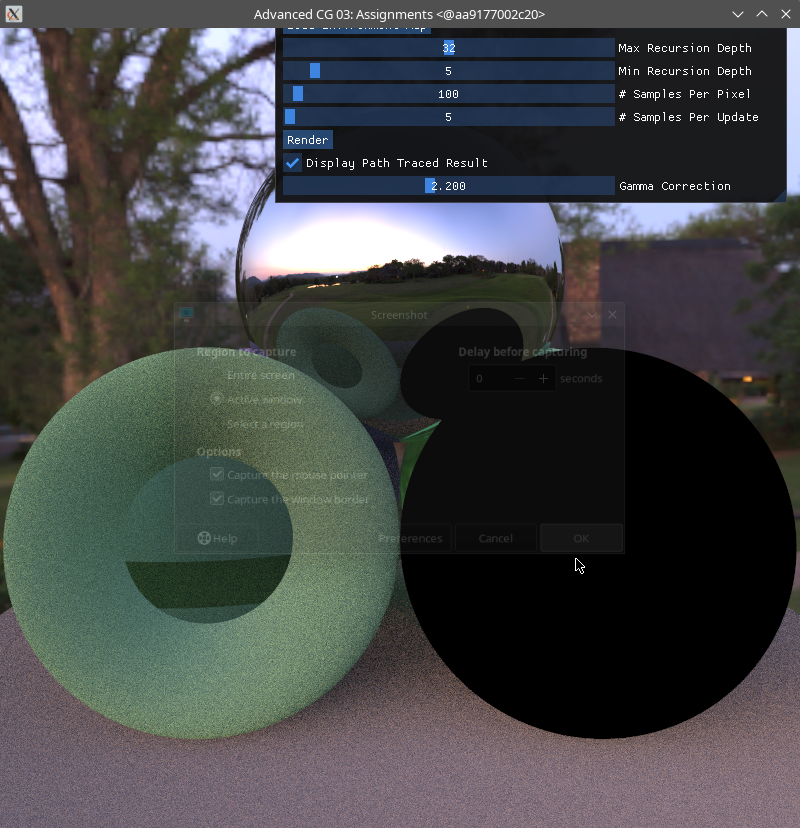
\includegraphics[width=10cm]{./advancedCG/figures/03kadai1.png}
 \end{center}
 \caption{課題1}
 \label{fig:kadai1}
\end{figure}

どちらも完成させることができなかった。\\

\section*{動作環境}
dockerで作成したdebian上で動作させた。
\lstinputlisting[caption=Dockerfile]{/home/pomu/sagyo/3d/Dockerfile}
\lstinputlisting[caption=Makefile]{/home/pomu/sagyo/3d/Makefile}
ホスト環境\\
OS:slackware 15.1\\
\begin{lstlisting}[caption=uname -aの実行結果]
Linux aya.home 6.1.57 #1 SMP PREEMPT_DYNAMIC Tue Oct 10 23:06:41 CDT 2023 x86_64 AMD Ryzen Threadripper 1950X 16-Core Processor AuthenticAMD GNU/Linux\\
\end{lstlisting}
実行したときに表示される情報\\
\begin{lstlisting}[caption=実行時の情報]

OpenGL version: 4.3 (Compatibility Profile) Mesa 20.3.5
GLSL version: 4.30
Vendor: nouveau
Renderer: NVE4

\end{lstlisting}
\end{document}
